\documentclass[12pt]{article}
\usepackage[utf8]{inputenc}
\usepackage[T1]{fontenc}

\usepackage{helvet}

\usepackage{subcaption}

\usepackage{graphicx}
\usepackage[export]{adjustbox}
\graphicspath{ { ./images/ } }

\title{\vspace{-5em}\textbf{Exploring Bitcoin Price Changes Relative to Software Indices}}
\author{James Alavosus}
\date{}

\begin{document}
\maketitle

\begin{center}
\LARGE \textbf{Background}
\end{center}

In the past few years, the cryptocurrency Bitcoin has made its way into the public eye. Once a niche internet currency used for various purposes, Bitcoin's dollar value shot up seemingly overnight, shifting its market position from a niche currency to a powerful investment opportunity. \par

\begin{figure}[h]
\centering
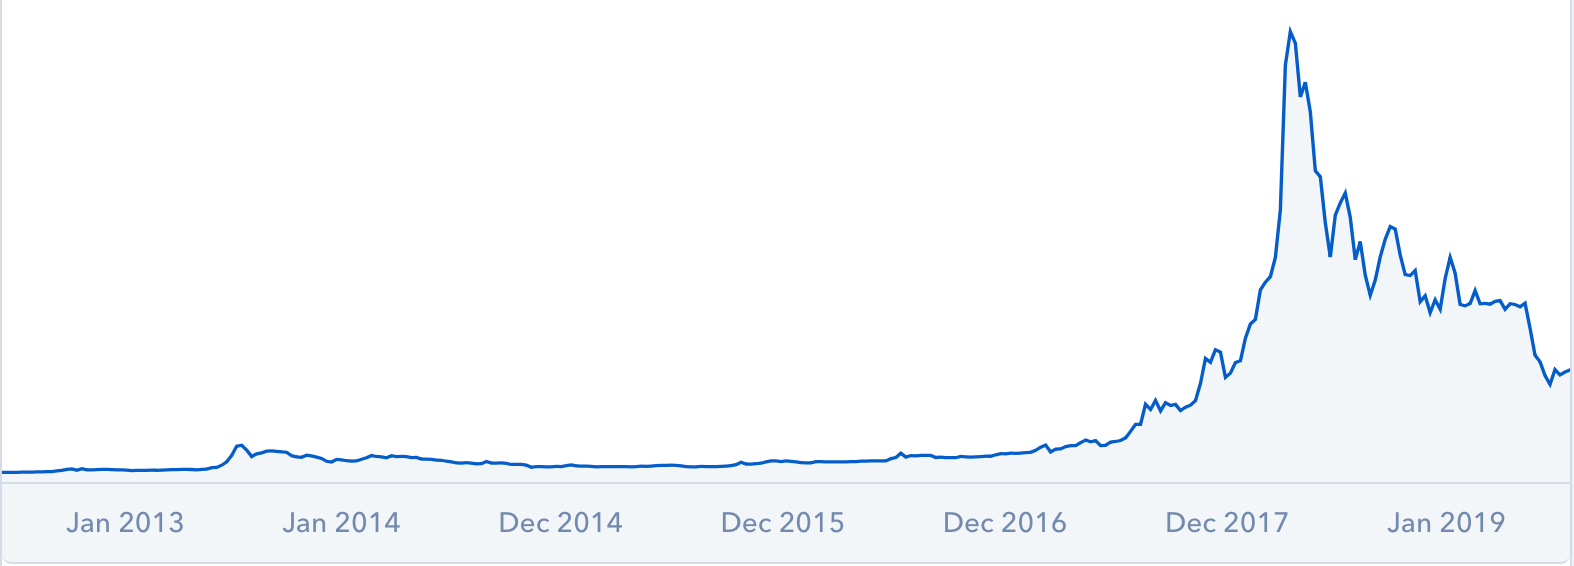
\includegraphics[width=0.75\textwidth]{images/btc-alltime-chart-coinbase.png} 
\caption{BTC Price Over Time (source: Coinbase)}
\end{figure}

In the investing world, a good measure of overall sector performance (ie. biotechnology, software, aviation) can be found by looking at the overall performance of one or more of those industries \textbf{\textit{indices}}. A sector index tracks the performance of a selection of stocks within a given sector, and bases its price on the overall average performance. \par

\begin{center}
\LARGE \textbf{Hypothesis}
\end{center}

Bitcoin, being at its core a software implementation, falls under the category of \textit{"Software"} for the purposes of overall sector performance tracking. As such, Bitcoin's percentage change should (in general) follow that of the \textbf{SPDR S\&P Software \& Services Index (XSW)}, as well as the \textbf{iShares Expanded Tech-Software Index (IGV)}.  

\pagebreak

\begin{center}
\LARGE \textbf{Data and Sources}
\end{center}

Historical OHLC (Open-High-Low-Close) data for IGV and XSW was scraped from Yahoo Finance (finance.yahooo.com) and converted to JSON. 
\\
Historical Bitcoin OHLC data was scraped from CoinMarketCap (coinmarketcap.com). All data was parsed using Python, using relevant third-party libraries when necessary, and all data visualization and charting was done using Tableau Desktop. 
\\ All historical data starts on December 27th, 2013, and ends at January 10th, 2019.

\begin{center}
\LARGE \textbf{Results}
\end{center}

Based on my charting, I can say that the change percentage of BTC \textit{somewhat} follows that of the software sector as a whole. 

\begin{figure}[h]
\begin{subfigure}{0.5\textwidth}	
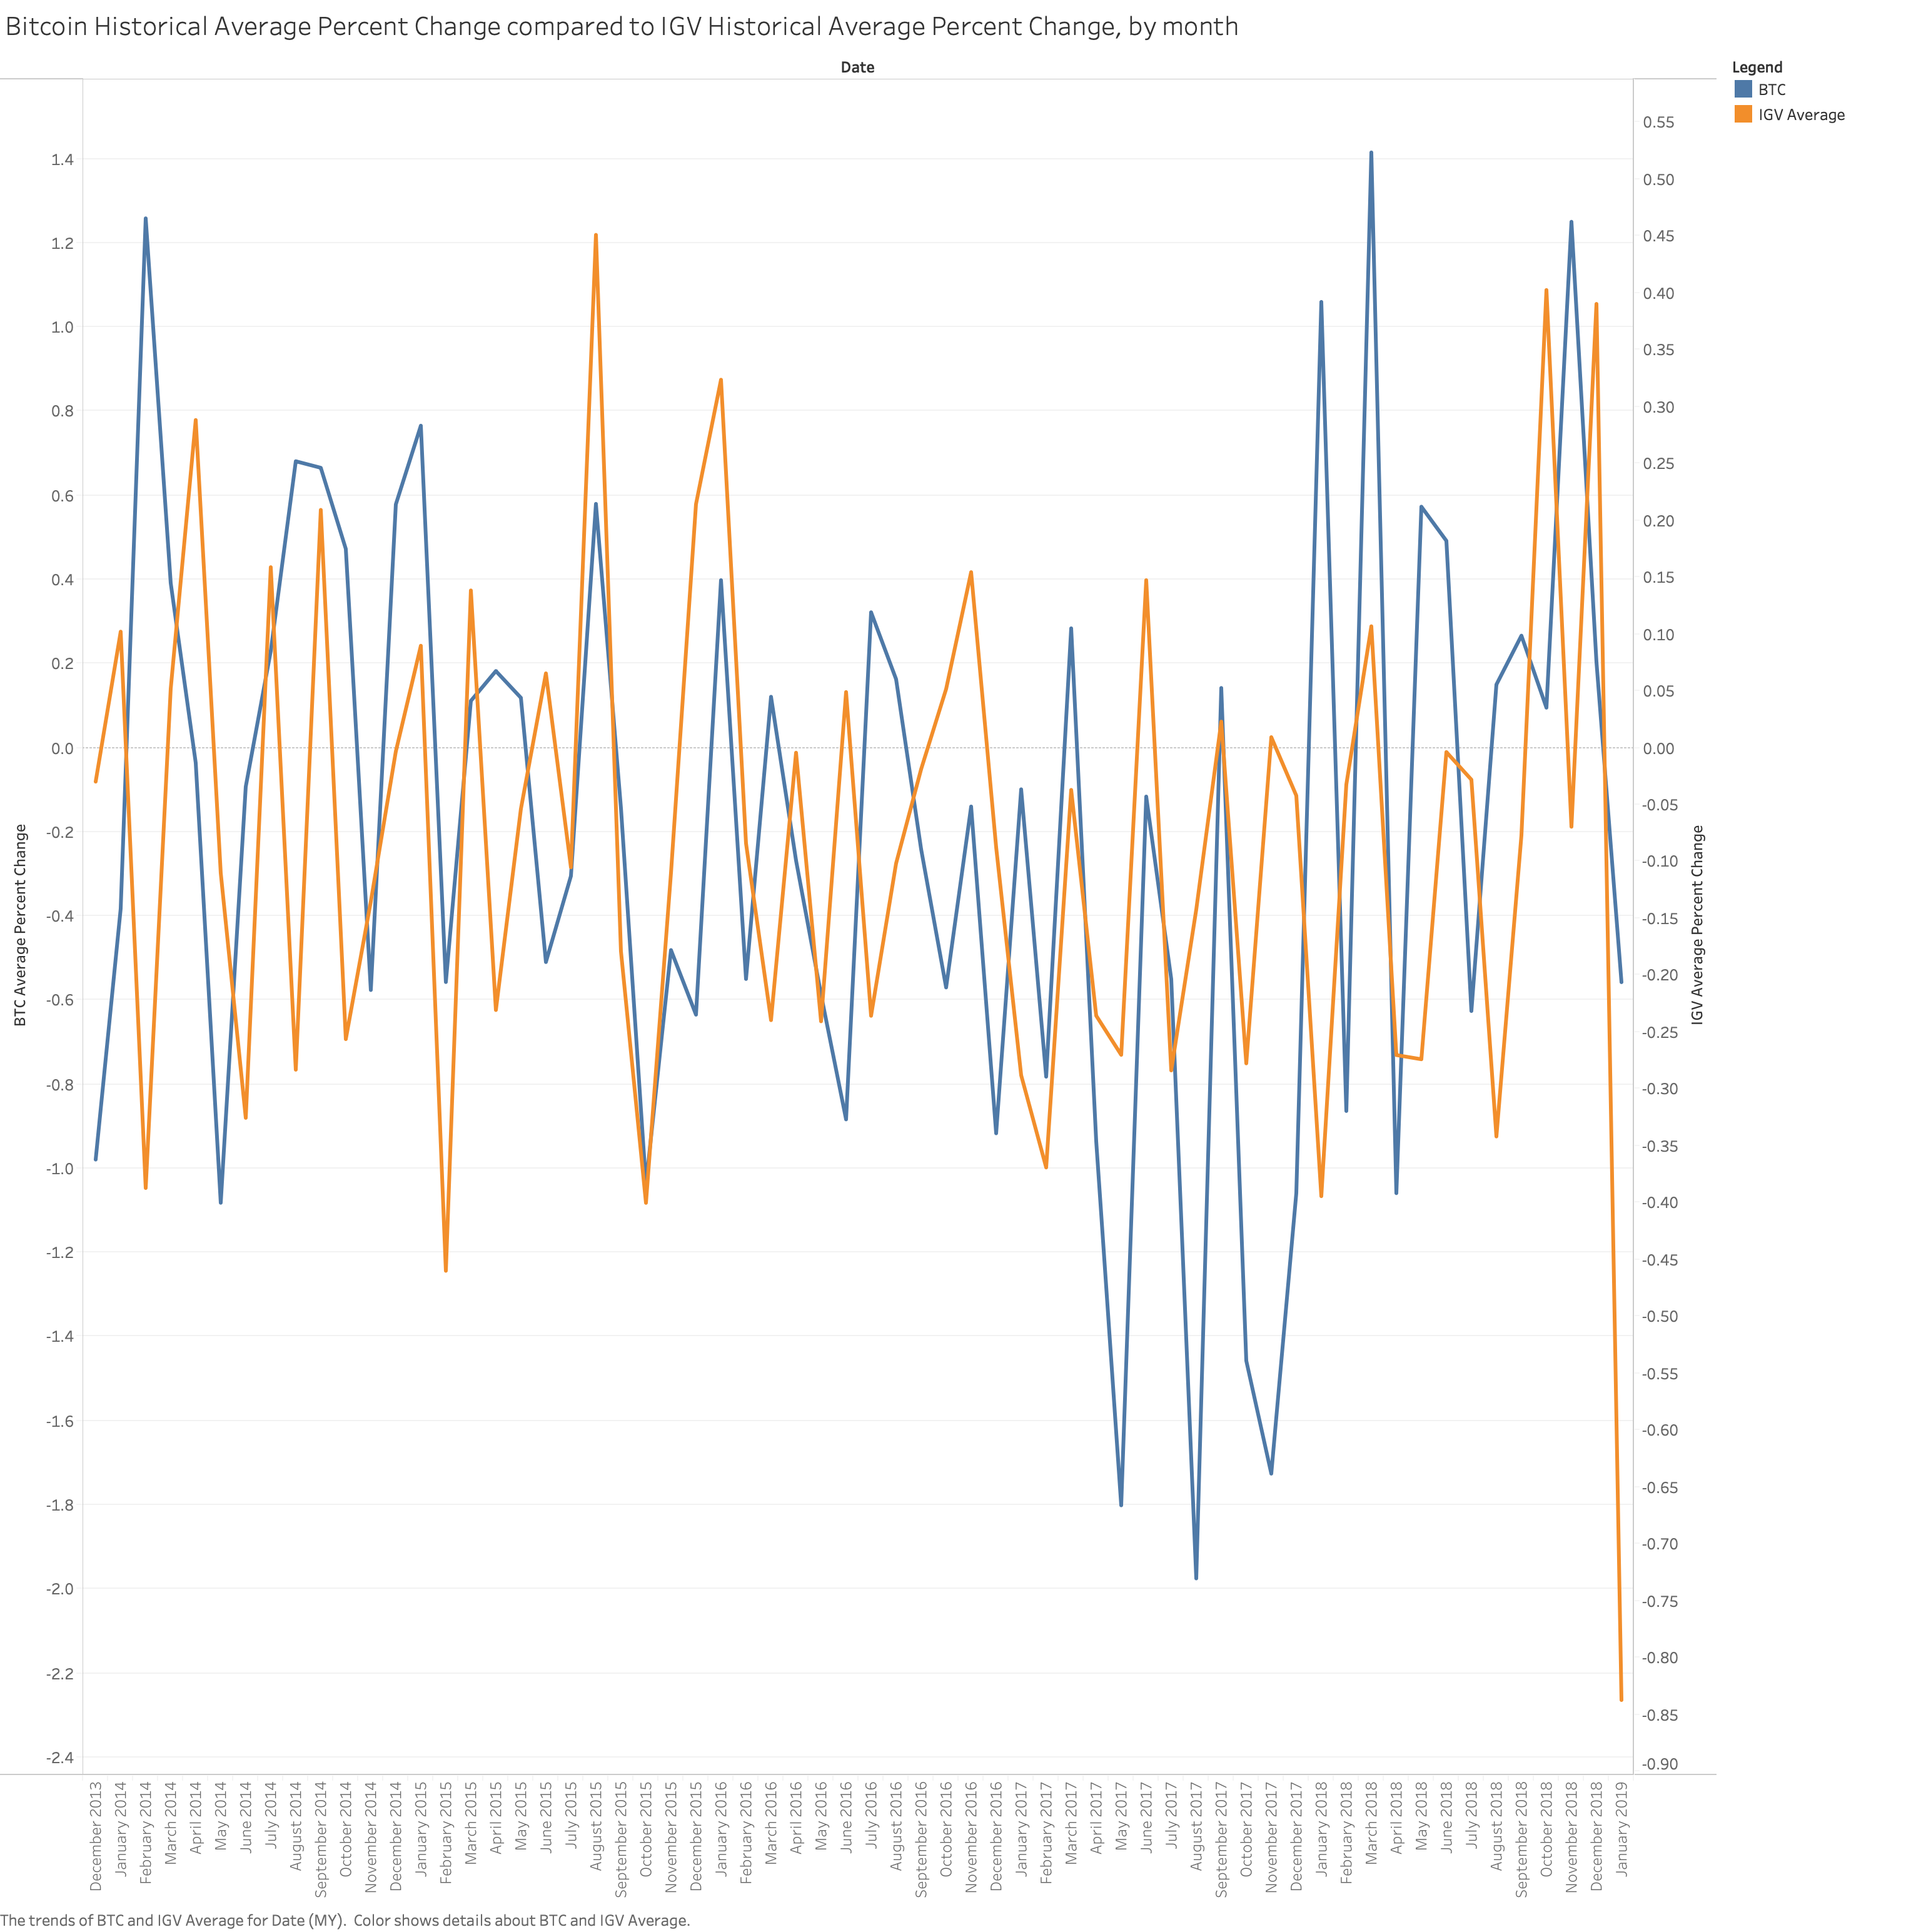
\includegraphics[width=0.9\linewidth, height=5cm]{images/BTC-IGV_avg_percent_change_chart.png}
\caption{BTC and IGV}
\end{subfigure}
\begin{subfigure}{0.5\textwidth}
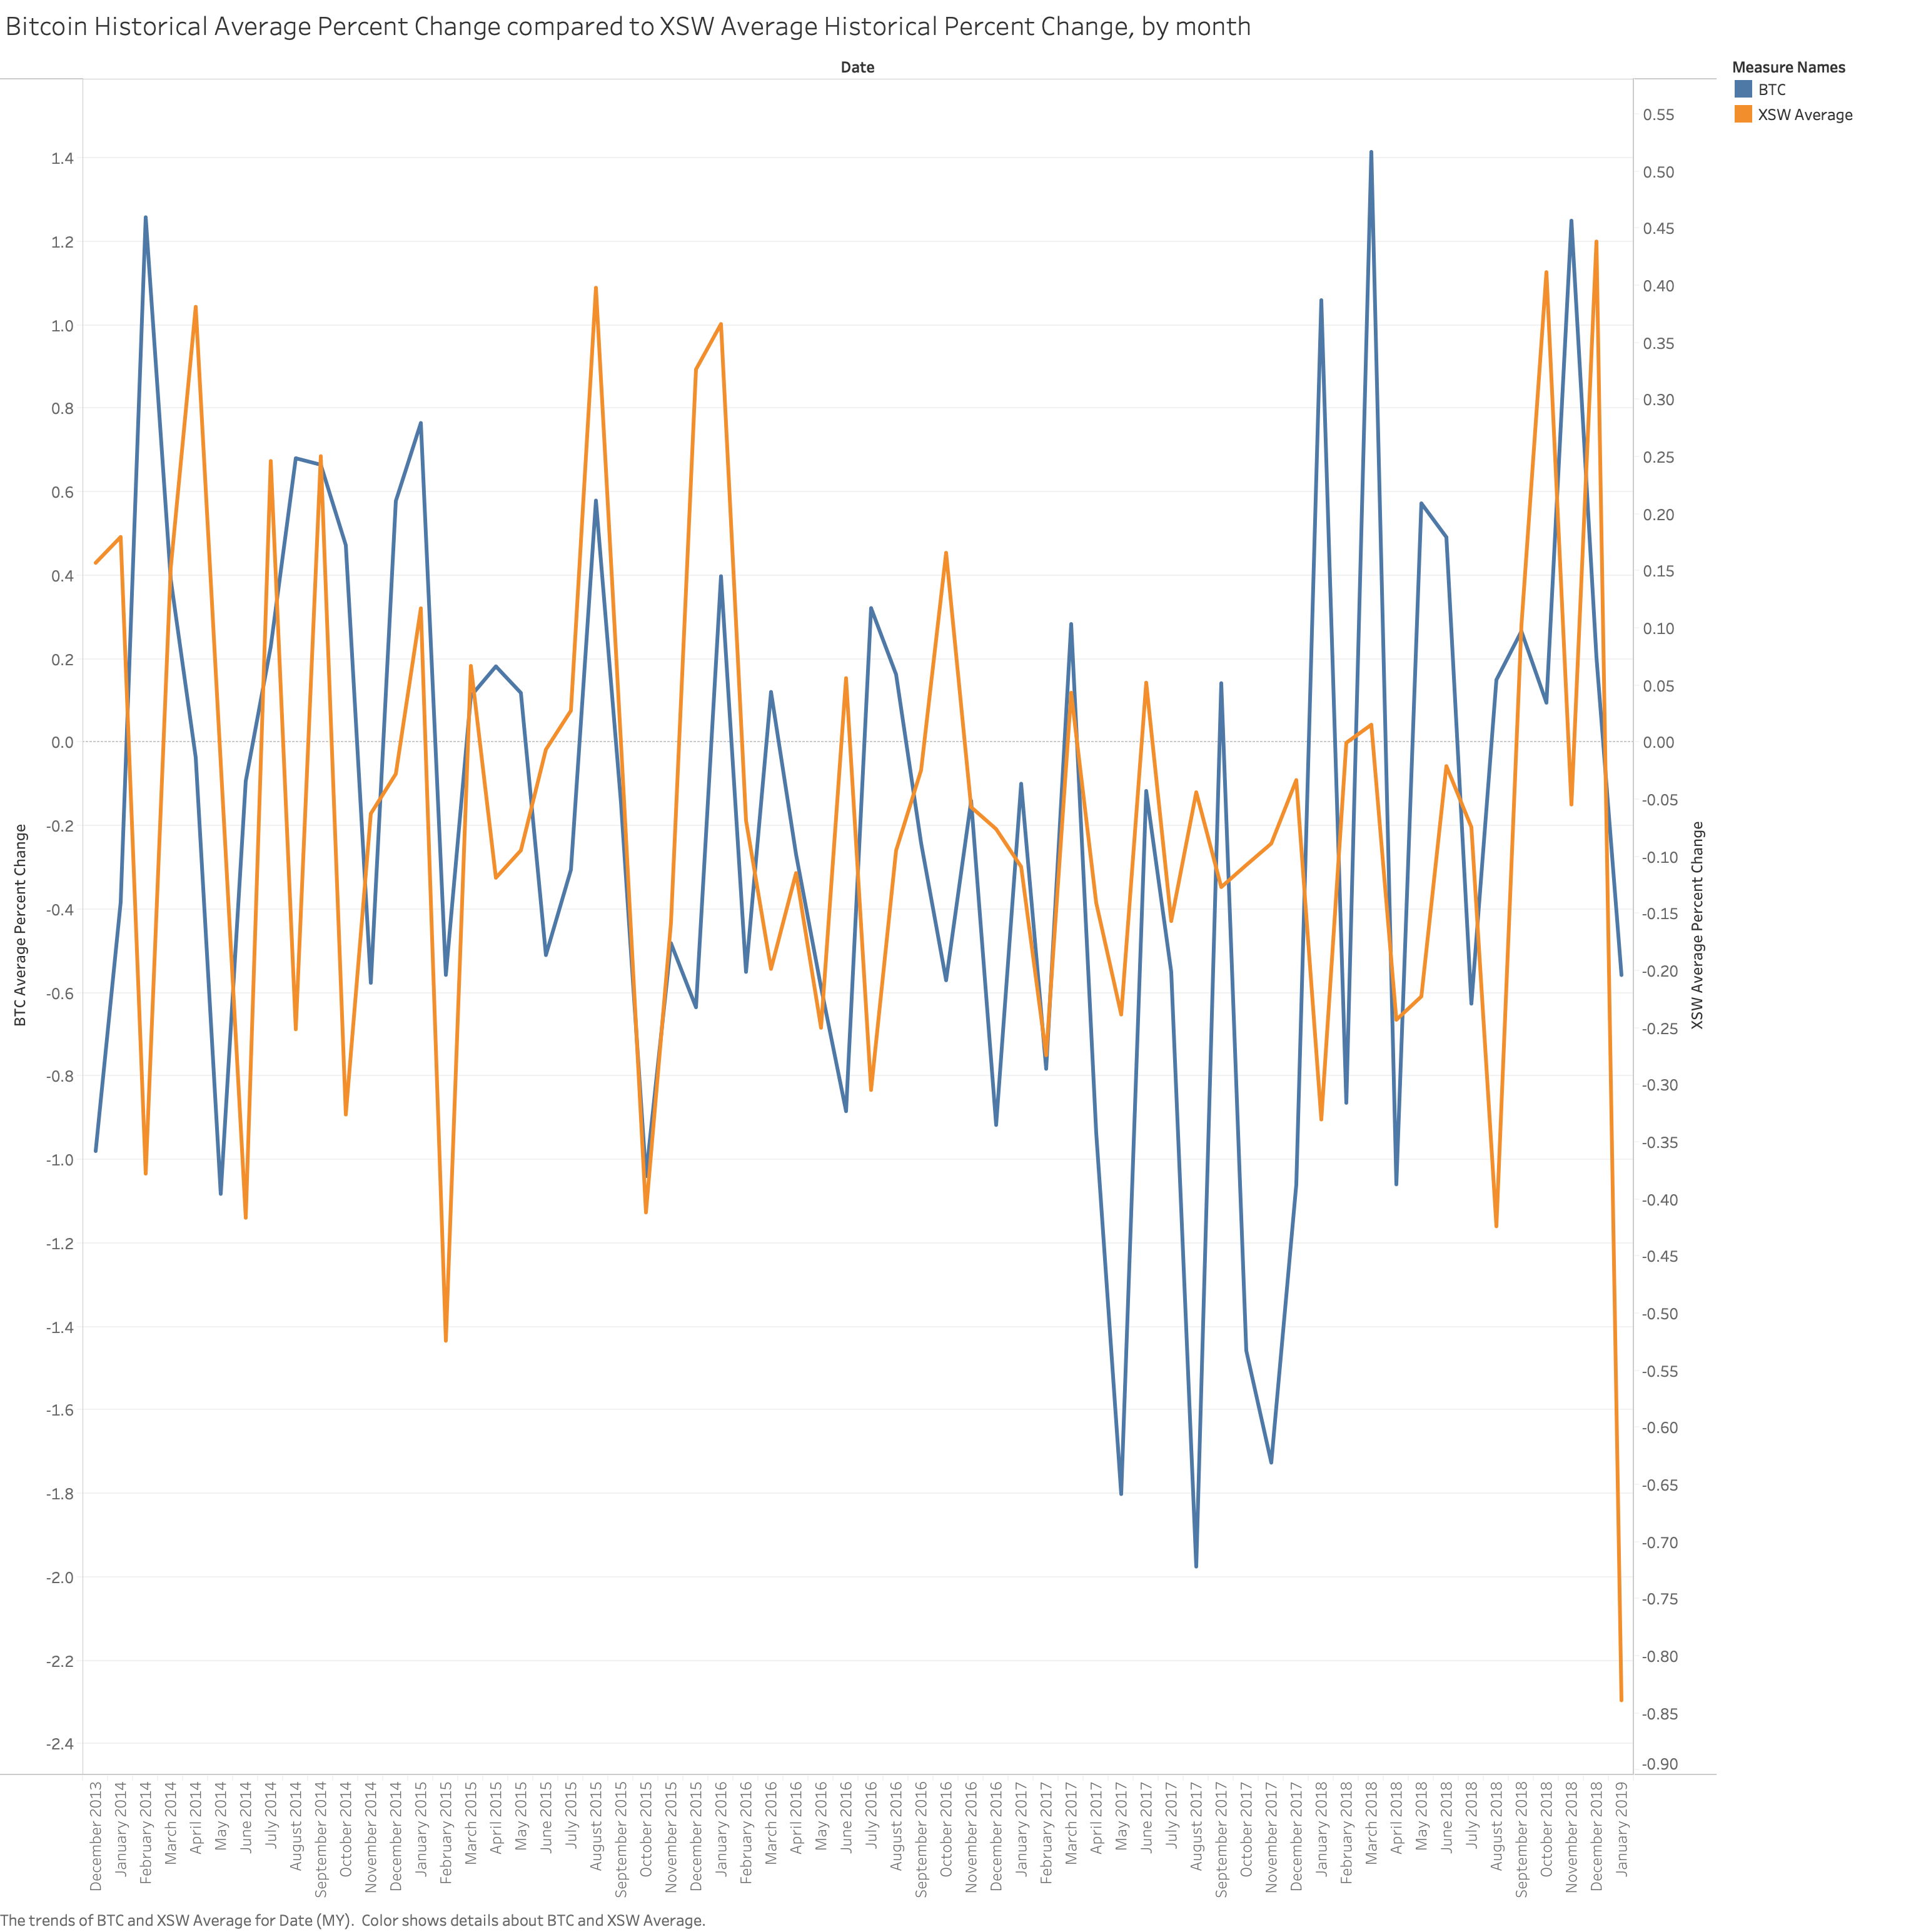
\includegraphics[width=0.9\linewidth, height=5cm]{images/BTC-XSW_avg_percent_change_chart.png}
\caption{BTC and XSW}
\end{subfigure}

\caption{Bitcoin Average Change Percentage Comparison}
\end{figure}

\par Each of these charts provides a slightly different view of the software sector's performance. From December 2013 to February 2017, we can see that Bitcoin on average performed around the same as the IGV and XSW indices. From February 2017 to November 2017, Bitcoin experienced quite the rollercoaster: three massive plunges, each followed by a correction. This pattern emerged again in January and February of 2018, when Bitcoin hit an all-time high price of \$16,776 USD per Bitcoin. These spikes don't appear to have a correlation to the software sector's overall performance.
\pagebreak \\
This month, January 2019, we can see Bitcoin's change percentage following the same downward trend (though not nearly the same percentage) as IGV and XSW. This plunge was preceeded by both the software sector and Bitcoin experiencing an average 0.45\% increase in value. 

\begin{center}
\LARGE \textbf{\\Conclusion}
\end{center}

Overall, my hypothesis that Bitcoin's performance would generally follow the performance of the software sector as a whole is \textit{plausible}. Aside from an extreme spike that occured in January and February 2018, Bitcoin does appear to follow the same performance trends of the IGV and XSW indices, and for the most part to the same change percentage. 

\begin{center}
\LARGE \textbf{\\ Notes and Sources}
\end{center}

\begin{flushleft}

\begin{large}
\textbf{Notes}
\end{large}

\begin{itemize}
\item Percent Change field was calculated using a short python script (percent\_change\_calculator.py). The math definitely isn't perfect.
\end{itemize}

\begin{large}
\textbf{Sources}
\end{large}

\begin{itemize}
\item Bitcoin historical data: https://coinmarketcap.com/currencies/bitcoin/historical-data/?start=20120101\&end=20190110
\item IGV historical data: https://finance.yahoo.com/quote/IGV/history?p=IGV\&.tsrc=fin-srch
\item XSW historical data: https://finance.yahoo.com/quote/XSW/history?p=XSW\&.tsrc=fin-srch
\end{itemize}

All code is available on Github, at https://github.com/jalavosus/data\_management\_final\_project

\end{flushleft}


\end{document} 